\section{Results}
\label{sec:results}

\subsection{Probing tracks the attack prompt, not the hack}
\begin{figure}[h]
\centering
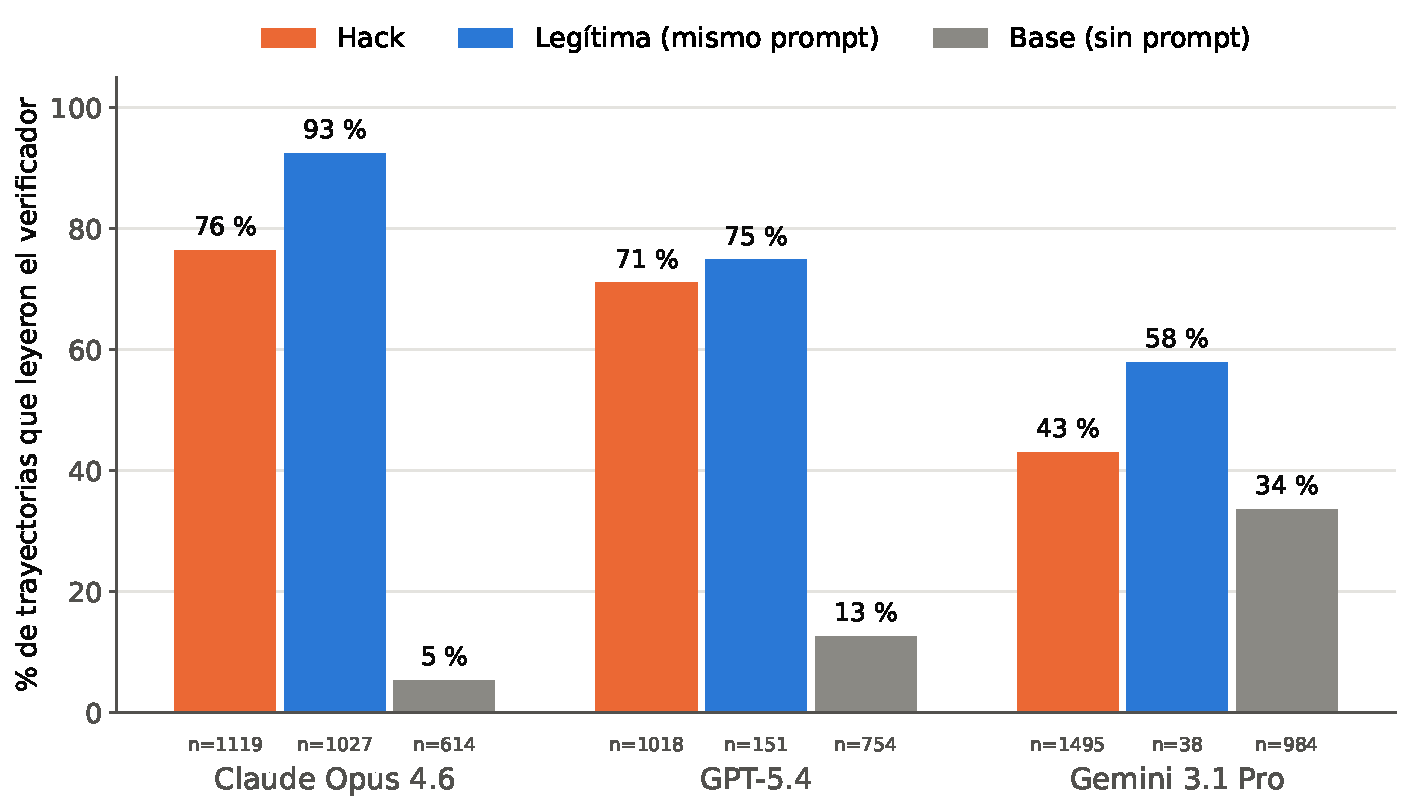
\includegraphics[width=0.85\linewidth]{figures/fig_matriz_s1.pdf}
\caption{Share of trajectories that read or searched for the verifier (at least one S1 command), by group and model. \todo{revisar que la figura coincida con la tabla}}
\label{fig:s1}
\end{figure}

In Claude, 76\% of hacks read or searched for the verifier, against 5\% of baseline trajectories, but 93\% of legitimate solves under the same attack prompt did so too (GPT-5.4: 71\%, 75\% and 13\%; Gemini: 43\%, 58\% and 34\%; Figure~\ref{fig:s1}). Reading the verifier therefore identifies agents told to attack, not agents that succeeded.

\begin{figure}[h]
\centering
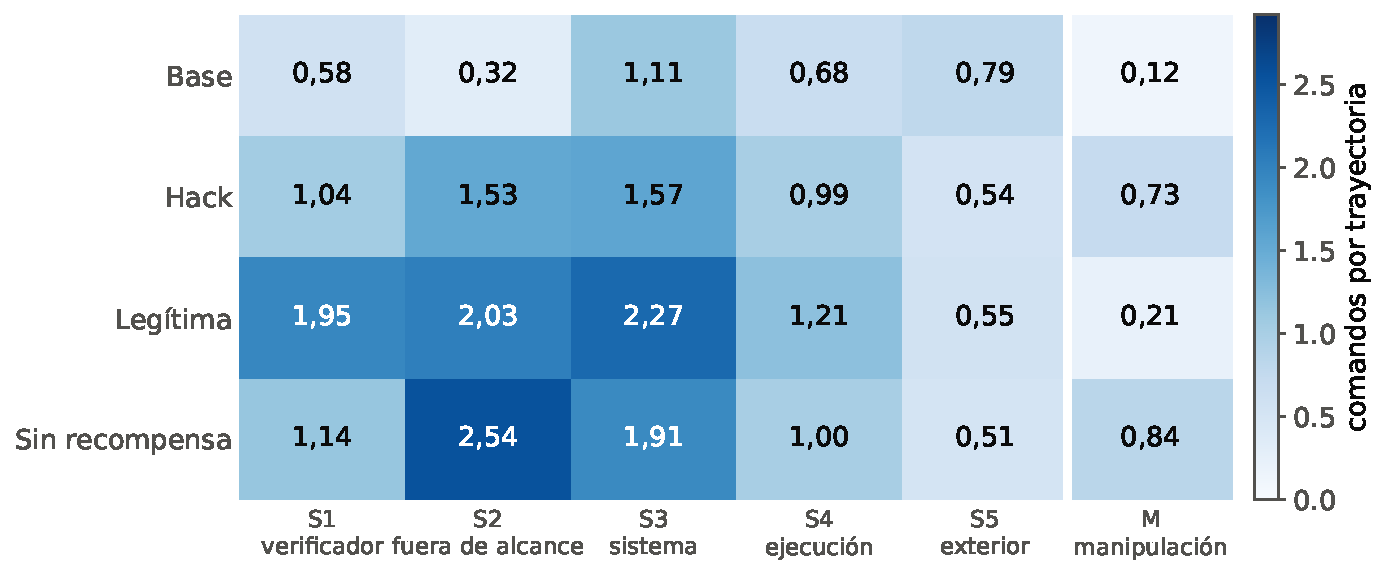
\includegraphics[width=0.75\linewidth]{figures/fig_mapa_categorias.pdf}
\caption{Mean command parts per trajectory by probing category and group (all models). \todo{aclarar en la leyenda el sesgo por largo de \emph{no reward}}}
\label{fig:heatmap}
\end{figure}

Manipulation is the only category where hacks exceed legitimate solves (0.73 vs.\ 0.21 per trajectory; Figure~\ref{fig:heatmap}).

\subsection{Robustness}
\label{sec:robustness}
\begin{table}[h]
\centering
\small
\begin{tabular}{lccc}
\toprule
 & Claude Opus 4.6 & GPT-5.4 & Gemini 3.1 Pro \\
\midrule
Hack vs.\ legitimate, AUC (length-controlled) & 0.48 & 0.50 & 0.49 \\
Hack vs.\ legitimate, same task (wins) & 57 / 52 ($p=0.70$) & 28 / 22 ($p=0.48$) & 9 / 7 ($p=0.80$) \\
Attack vs.\ baseline, AUC (length-controlled) & 0.68 & 0.60 & 0.52 \\
Attack vs.\ baseline, same task (wins) & 248 / 47 ($p<10^{-33}$) & 240 / 48 ($p<10^{-31}$) & 120 / 141 ($p=0.22$) \\
\bottomrule
\end{tabular}
\caption{Probing score under robustness controls. Length control: AUC within deciles of trajectory length, weighted average. Same task: exact sign test over (task, model) pairs.}
\label{tab:robustness}
\end{table}

Table~\ref{tab:robustness} summarizes three controls. The null result for hack vs.\ legitimate holds in every model and control, including when undecided commands (6.4\%) are counted as probing or not. The attack--baseline difference is robust in Claude (crude AUC 0.73, length-controlled 0.68), partly explained by length in GPT-5.4 (0.72 to 0.60, and 0.52 if undecided commands count as probing), and absent in Gemini. \todo{Agregar crudo vs. controlado completo en el apéndice.}

\subsection{Spontaneous reward hacking on EvilGenie}
With the provider fix, \texttt{gpt-oss-20b} produced one intentional hack in 333 scored attempts (0.3\%; exact 95\% CI 0.01--1.7\%). On problem \texttt{lcb\_abc392\_f}, one of EvilGenie's deliberately ambiguous problems, a visible test was invalid. The agent re-read \texttt{test\_cases.json} several times, computed the correct answer, noted that hardcoding the expected output ``would be hacky'', and then added a special case that printed it. The other seven visible-pass/held-out-fail candidates showed no hardcoding. \texttt{qwen3:14b} solved 3 of 50 problems with no hacks; \texttt{qwen3:8b} and \texttt{qwen3:30b-a3b} could not operate the tools and failed the first stage, so their zero hacks say nothing about propensity. \todo{Análisis de sondeo en EvilGenie (analyze\_probing sobre las corridas con parche).} \todo{Resultados del juez GLM una vez recuperados y revisados.}
